\documentclass{beamer}
\mode<presentation>
\usepackage{amsmath,amssymb,mathtools}
\usepackage{textcomp}
\usepackage{gensymb}
\usepackage{adjustbox}
\usepackage{subcaption}
\usepackage{enumitem}
\usepackage{multicol}
\usepackage{listings}
\usepackage{url}
\usepackage{graphicx} % <-- needed for images
\def\UrlBreaks{\do\/\do-}

\usetheme{Boadilla}
\usecolortheme{lily}
\setbeamertemplate{footline}{
  \leavevmode%
  \hbox{%
  \begin{beamercolorbox}[wd=\paperwidth,ht=2ex,dp=1ex,right]{author in head/foot}%
    \insertframenumber{} / \inserttotalframenumber\hspace*{2ex}
  \end{beamercolorbox}}%
  \vskip0pt%
}
\setbeamertemplate{navigation symbols}{}

\lstset{
  frame=single,
  breaklines=true,
  columns=fullflexible,
  basicstyle=\ttfamily\tiny   % tiny font so code fits
}

\numberwithin{equation}{section}

% ---- your macros ----
\providecommand{\nCr}[2]{\,^{#1}C_{#2}}
\providecommand{\nPr}[2]{\,^{#1}P_{#2}}
\providecommand{\mbf}{\mathbf}
\providecommand{\pr}[1]{\ensuremath{\Pr\left(#1\right)}}
\providecommand{\qfunc}[1]{\ensuremath{Q\left(#1\right)}}
\providecommand{\sbrak}[1]{\ensuremath{{}\left[#1\right]}}
\providecommand{\lsbrak}[1]{\ensuremath{{}\left[#1\right.}}
\providecommand{\rsbrak}[1]{\ensuremath{\left.#1\right]}}
\providecommand{\brak}[1]{\ensuremath{\left(#1\right)}}
\providecommand{\lbrak}[1]{\ensuremath{\left(#1\right.}}
\providecommand{\rbrak}[1]{\ensuremath{\left.#1\right)}}
\providecommand{\cbrak}[1]{\ensuremath{\left\{#1\right\}}}
\providecommand{\lcbrak}[1]{\ensuremath{\left\{#1\right.}}
\providecommand{\rcbrak}[1]{\ensuremath{\left.#1\right\}}}
\theoremstyle{remark}
\newtheorem{rem}{Remark}
\newcommand{\sgn}{\mathop{\mathrm{sgn}}}
\providecommand{\abs}[1]{\left\vert#1\right\vert}
\providecommand{\res}[1]{\Res\displaylimits_{#1}}
\providecommand{\norm}[1]{\lVert#1\rVert}
\providecommand{\mtx}[1]{\mathbf{#1}}
\providecommand{\mean}[1]{E\left[ #1 \right]}
\providecommand{\fourier}{\overset{\mathcal{F}}{ \rightleftharpoons}}
\providecommand{\system}{\overset{\mathcal{H}}{ \longleftrightarrow}}
\providecommand{\dec}[2]{\ensuremath{\overset{#1}{\underset{#2}{\gtrless}}}}
\newcommand{\myvec}[1]{\ensuremath{\begin{pmatrix}#1\end{pmatrix}}}
\newcommand{\mydet}[1]{\ensuremath{\begin{vmatrix}#1\end{vmatrix}}}

\newenvironment{amatrix}[1]{%
  \left(\begin{array}{@{}*{#1}{c}|*{#1}{c}@{}}
}{%
  \end{array}\right)
}

\newcommand{\myaugvec}[2]{\ensuremath{\begin{amatrix}{#1}#2\end{amatrix}}}
\let\vec\mathbf
% ---------------------

\title{Matgeo Presentation - Problem 5.9.10}
\author{EE25BTECH11048 - Revanth Siva Kumar.D}

\begin{document}

\begin{frame}
  \titlepage
\end{frame}

\begin{frame}{Problem Statement}
The present age of a father is three years more than three times the age of his son. Three years hence the father's age will be 10 years more than twice the age of the son. Determine their present ages.

\end{frame}

\begin{frame}{Data}

\begin{table}[h!]
  \centering
  \begin{tabular}{|c|c|}
\hline
\textbf{Name} & \textbf{Value} \\ \hline
$\vec{A}$ & $\myvec{2 & 1 \\0 & 3}$ \\ \hline
\end{tabular}

  \caption*{Table : Equations}
  \label{5.9.2}
\end{table}

\end{frame}

\begin{frame}{Solution}


Let 
\[
x = \text{son's present age}, \quad y = \text{father's present age}.
\]

From the problem statement:

1. \textbf{Father's present age is three years more than three times son's age}:
\[
y = 3x + 3 \quad \Rightarrow \quad -3x + y = 3
\]

2. \textbf{Three years hence, father's age will be 10 years more than twice son's age}:
\[
y + 3 = 2(x+3) + 10 \quad \Rightarrow \quad -2x + y = 13
\]
Writing in matrix form:

\begin{align}
\myvec{-3 & 1\\-2 & 1}\myvec{x\\y} &= \myvec{3\\13}
\end{align}
\end{frame}
\begin{frame}{Solution}

Forming the augmented matrix:

\begin{align}
\myaugvec{2}{-3 & 1 & 3\\-2 & 1 & 13}
\end{align}

Using Gaussian elimination:
\begin{align}
\myaugvec{2}{-3 & 1 & 3\\-2 & 1 & 13} 
\xleftrightarrow{\;R_2 \to R_2 - \frac{2}{3}R_1\;}
\myaugvec{2}{-3 & 1 & 3\\0 & \frac{1}{3} & 11}
\end{align}
Back substitution gives:
\begin{align}
\frac{y}{3} &= 11 \\
y &= 33\\
-3x + y &= 3 \;\Rightarrow\; -3x + 33 = 3 \;\Rightarrow\; x = 10
\end{align}

\begin{align}
\myvec{x\\y} &= \myvec{10\\33}
\end{align}
\end{frame}

\begin{frame}{Conclusion}
Therefore, the present ages are:

\begin{align*}
\text{Son's age } &= 10 \text{ years} \\
\text{Father's age } &= 33 \text{ years}
\end{align*}
\end{frame}
\begin{frame}[fragile]{C code}
\begin{lstlisting}
#include <stdio.h>

double *gaussian_elimination(double a[2][3]) {

  static double sol[2];
  int i, j, k;
  double ratio;
  int n = 2;

  // forward elimination (j for rows and i for columns of augmented_matrix,)
  for (i = 0; i < n - 1; i++) {

    for (j = i + 1; j < n; j++) {
      ratio = a[j][i] / a[i][i];

      for (k = i; k < n + 1; k++) { // k is also for columns
        a[j][k] -=
            ratio *
            a[i][k]; // to do R2 -> R2 - ratio*R1 , then R3 -> R3 -ratio*R1
      }
    }
  }
\end{lstlisting}
\end{frame}
\begin{frame}[fragile]{C Code}
\begin{lstlisting}
 // Back substitution
  for (i = n - 1; i >= 0; i--) {

    sol[i] = a[i][n];

    for (j = i + 1; j < n; j++) {
      sol[i] -= a[i][j] * sol[j];
    }

    sol[i] /= a[i][i];
  }

  return sol;
}

int main() {
    // Augmented matrix for the father-son problem: -3x + y = 3, -2x + y = 13
    double a[2][3] = {
        {-3, 1, 3},
        {-2, 1, 13}
    };

    double *solution = gaussian_elimination(a);

    printf("Son's age (x) = %.2lf\n", solution[0]);
    printf("Father's age (y) = %.2lf\n", solution[1]);

    return 0;
}
\end{lstlisting}
\end{frame}
\begin{frame}[fragile]{Python shared output}
\begin{lstlisting}
import ctypes
import sys
import os
import numpy as np
import matplotlib.pyplot as plt

# save figure in figs folder
figs_folder = os.path.join("..", "figs")
os.makedirs(figs_folder, exist_ok=True)  # create folder if it doesn't exist

# load the shared object
lib = ctypes.CDLL("./points.so")

# define return type and arg type
lib.gaussian_elimination.restype = ctypes.POINTER(ctypes.c_double)
lib.gaussian_elimination.argtypes = [((ctypes.c_double * 3) * 2)]

# define augmented matrix for father-son problem
# -3x + y = 3
# -2x + y = 13
a = ((ctypes.c_double * 3) * 2)()
a[0][:] = [-3.0, 1.0, 3.0]
a[1][:] = [-2.0, 1.0, 13.0]

# call the C function
sol = lib.gaussian_elimination(a)
solution = [sol[i] for i in range(2)]
x, y = solution
print("Solution from C:", solution)
\end{lstlisting}
\end{frame}
\begin{frame}[fragile]{Python shared output}
\begin{lstlisting}
# create x range for plotting
x_vals = np.linspace(0, 15, 100)

# equations solved for y
y1 = 3 * x_vals + 3       # from y = 3x + 3
y2 = 2 * x_vals + 13  # from y + 3 = 2(x+3)+10 → y = 2x + 13

# plotting
plt.figure(figsize=(8, 6))

# plot the lines
plt.plot(x_vals, y1, label="y = 3x + 3", color="green")
plt.plot(x_vals, y2, label="y = 2x + 13", color="blue")

# plot the solution point
plt.scatter(x, y, color="red", label=f"P({x:.2f},{y:.2f})")
plt.text(x + 0.3, y + 0.3, f"P({x:.2f},{y:.2f})", fontsize=10, color="red")

# labels and grid
plt.xlabel("X axis (Son's Age)")
plt.ylabel("Y axis (Father's Age)")
plt.title("Father-Son Age Problem: Intersection Point")
plt.legend()
plt.grid(True)

# save figure
plt.tight_layout()
plt.savefig(os.path.join(figs_folder, "solution.png"))
plt.show()

\end{lstlisting}
    
\end{frame}
\begin{frame}[fragile]{PYTHON plot.py}
\begin{lstlisting}
    import os
import numpy as np
import matplotlib.pyplot as plt

# save figure in figs folder
figs_folder = os.path.join("..", "figs")
os.makedirs(figs_folder, exist_ok=True)  # create folder if it doesn't exist

# solve system of equations directly using numpy
# -3x + y = 3
# -2x + y = 13
A = np.array([[-3, 1],
              [-2, 1]], dtype=float)

b = np.array([3, 13], dtype=float)

solution = np.linalg.solve(A, b)
x, y = solution
print("Solution from Python:", solution)

# create x range for plotting
x_vals = np.linspace(0, 15, 100)

# equations solved for y
y1 = 3 * x_vals + 3      # from y = 3x + 3
y2 = 2 * x_vals + 13 - 2*x_vals? let's compute properly
# original equation: -2x + y = 13 → y = 2x + 13

y2 = 2 * x_vals + 13     # from -2x + y = 13 → y = 2x + 13
\end{lstlisting}
\end{frame}
\begin{frame}[fragile]{PYTHON plot.py}
\begin{lstlisting}
# plotting
plt.figure(figsize=(8, 6))

# plot the lines
plt.plot(x_vals, y1, label="y = 3x + 3", color="green")
plt.plot(x_vals, y2, label="y = 2x + 13", color="blue")

# plot the solution point
plt.scatter(x, y, color="red", label=f"P({x:.2f},{y:.2f})")
plt.text(x + 0.3, y + 0.3, f"P({x:.2f},{y:.2f})", fontsize=10, color="red")

# labels and grid
plt.xlabel("X axis (Son's Age)")
plt.ylabel("Y axis (Father's Age)")
plt.title("Father-Son Age Problem: Intersection Point")
plt.legend()
plt.grid(True)

# save figure
plt.tight_layout()
plt.savefig(os.path.join(figs_folder, "solution.png"))
plt.show()

\end{lstlisting}
    
\end{frame}
\begin{frame}{Plot}

\begin{figure}[h!]
  \centering
  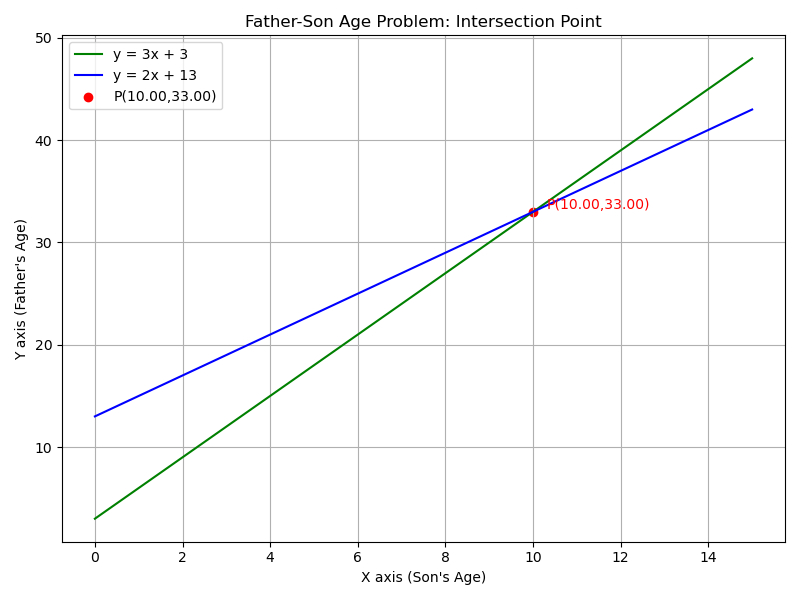
\includegraphics[width=0.7\columnwidth]{figs/Figure_1.png} 
   \caption*{Fig : Lines}
  \label{Fig1}
\end{figure}

\end{frame}

\end{document}